\section{Tarefas de Processamento}
Como explicado, o APPA ira gerenciar nossas tarefas de processamento, ja foi abordado também alguns atributos que serão necessários para 14BIS executar os modelos lógicos. Tendo isso em vista é necessário que seja implementado \textit{scripts} de mineração e pré-processamento para que a base de dados de dados do projeto tenha a estrutura necessária para que as IAs possam agir.

Essa sessão tem como objetivo detalhar os atributos e \textit{scripts} criados para gerar-los. Além disso em alguns casos, onde são utilizados recursos externos como APIs, será detalhado a configuração necessária.

É importante ressaltar que todo o projeto é \textit{Open Source}, conhecidos como projeto de código aberto, e todo o código criado para esse projeto pode ser encontrado na plataforma de versionamento do GitHub\footnote{\url{https://github.com/getdumont}}.

Antes de iniciarmos as explicações é necessário que para reprodução dessa pesquisa você tenha inicialmente o Docker\footnote{\url{https://www.docker.com/}} instalado. Caso deseje executar as tarefas individualmente, como será citado aqui, é necessário que você tenha instalado na sua máquina o Python 3.6\footnote{\url{https://www.python.org/downloads/release/python-360/}} e o NodeJS 9.11\footnote{\url{https://nodejs.org/en/blog/release/v9.11.1/}}. Vale lembrar que todo código aqui demonstrado foi escrito, executado e testado em um sistema operacional com base Unix, logo a portabilidade com Windows não é garantida.

Uma vez com as ferramentas instaladas no sistema operacional, torna-se possível a reprodução dessa pesquisa. A primeira etapa como já discursada até então se refere a coleta de dados.

\subsection{Tarefa de Coleta}
A coleta será feita utilizando a API publica do twitter, o link para a documentação é \url{https://developer.twitter.com/en/docs}. Será trabalhado no projeto duas entidades: Tweet e Usuário. O tweet é a entidade que representa a publicação do usuário, enquanto o usuário contém informações necessárias sobre o seu perfil.

Para que seja possível acessar a API é necessário criar uma conta de desenvolvimento e gerar o \textit{token} de acesso\footnote{\url{https://apps.twitter.com/app/new}}. Com a chave em mãos é possível replicar o arquivo /collector/client/.env\_sample dentro do projeto Dumont para /collector/client/.env, e conforme demonstrado na figura \ref{fig:twitteropts}, completar os campos necessários.

Para rodar basta executar o comando \textit{node collector/twitter.js}, e verá a saída de dados. Existem duas observações relevantes a serem feitas nessa etapa:
\begin{itemize}
  \item !AppaTag(tweet) e !AppaTag(user): Se notar, algumas linhas começarão com essas duas anotações, são essas anotações que serão responsáveis por fazer com que o APPA identifique qual entidade de processamento será responsável por processar cada tipo de dado.
  \item Dados de Emoji: É possível notar que alguns dados mapeados não existem na API do Twitter. Como observado, um dos problemas durante a mineração de dados é o uso de \textit{emojis} em textos, já citado também, é possível algumas tarefas de pré-processamento serem executadas durante a própria coleta. Sabendo que emojis podem expressar sentimentos \cite{novak2015sentiment}, e que armazenar e tratar esse dado poderia ser relevante na hora de confirmar sentimento em frases, o autor também criou a biblioteca \textit{Emojinator}\footnote{https://github.com/getdumont/emojinator}, além do texto tradado, também será obtida informações do \textit{emojis} utilizados no meio do texto.
\end{itemize}

\begin{figure}
    \centering
    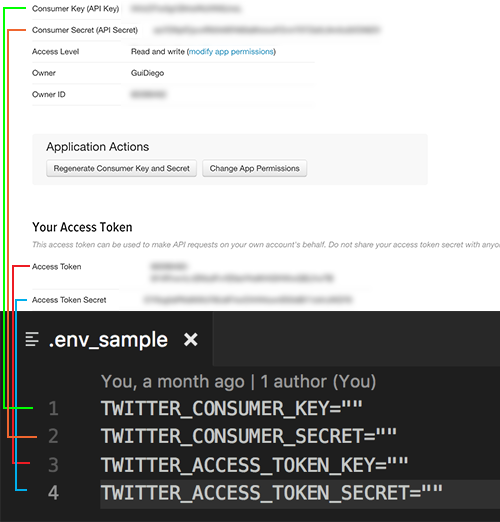
\includegraphics[width=.8\textwidth]{imagens/twitteropts.png}
    \caption{Imagem demonstrando onde cada chave deve ser inserida no código}
    \label{fig:twitteropts}
\end{figure}

Uma vez configurado o coletor, ainda é necessário entender e configurar as outras tarefas para que o APPA funcione apropriadamente, logo, é necessário entender como essas entidades ficarão no final e quais as tarefas que realizarão essa manipulação.

